% ---
% draft: false
% tags: ["math", "research", "Physics"]
% ---

\documentclass{pensee}

\title{My First Academic Blog Post}
\author{}
\date{2026-05-22}

\begin{document}

\section{Introduction}
\subsection{Physics}
\subsubsection{The Special Theory of Relativity}
This is my blog post with some math.

\paragraph{Moving body}
This is the first subject.
\subparagraph{Electricitys} It's my second paragraph.


\begin{equation}
  E = mc^2
\end{equation}

\begin{equation}
  e^{-i \pi} + 1 = 0
\end{equation}

\begin{equation}
  a^2 + b^2 = c^2
\end{equation}

\begin{equation}
	sin^2(x) + cos^2(x) = 1
\end{equation}


A historic group photo:

\begin{figure}[H]
    \centering
    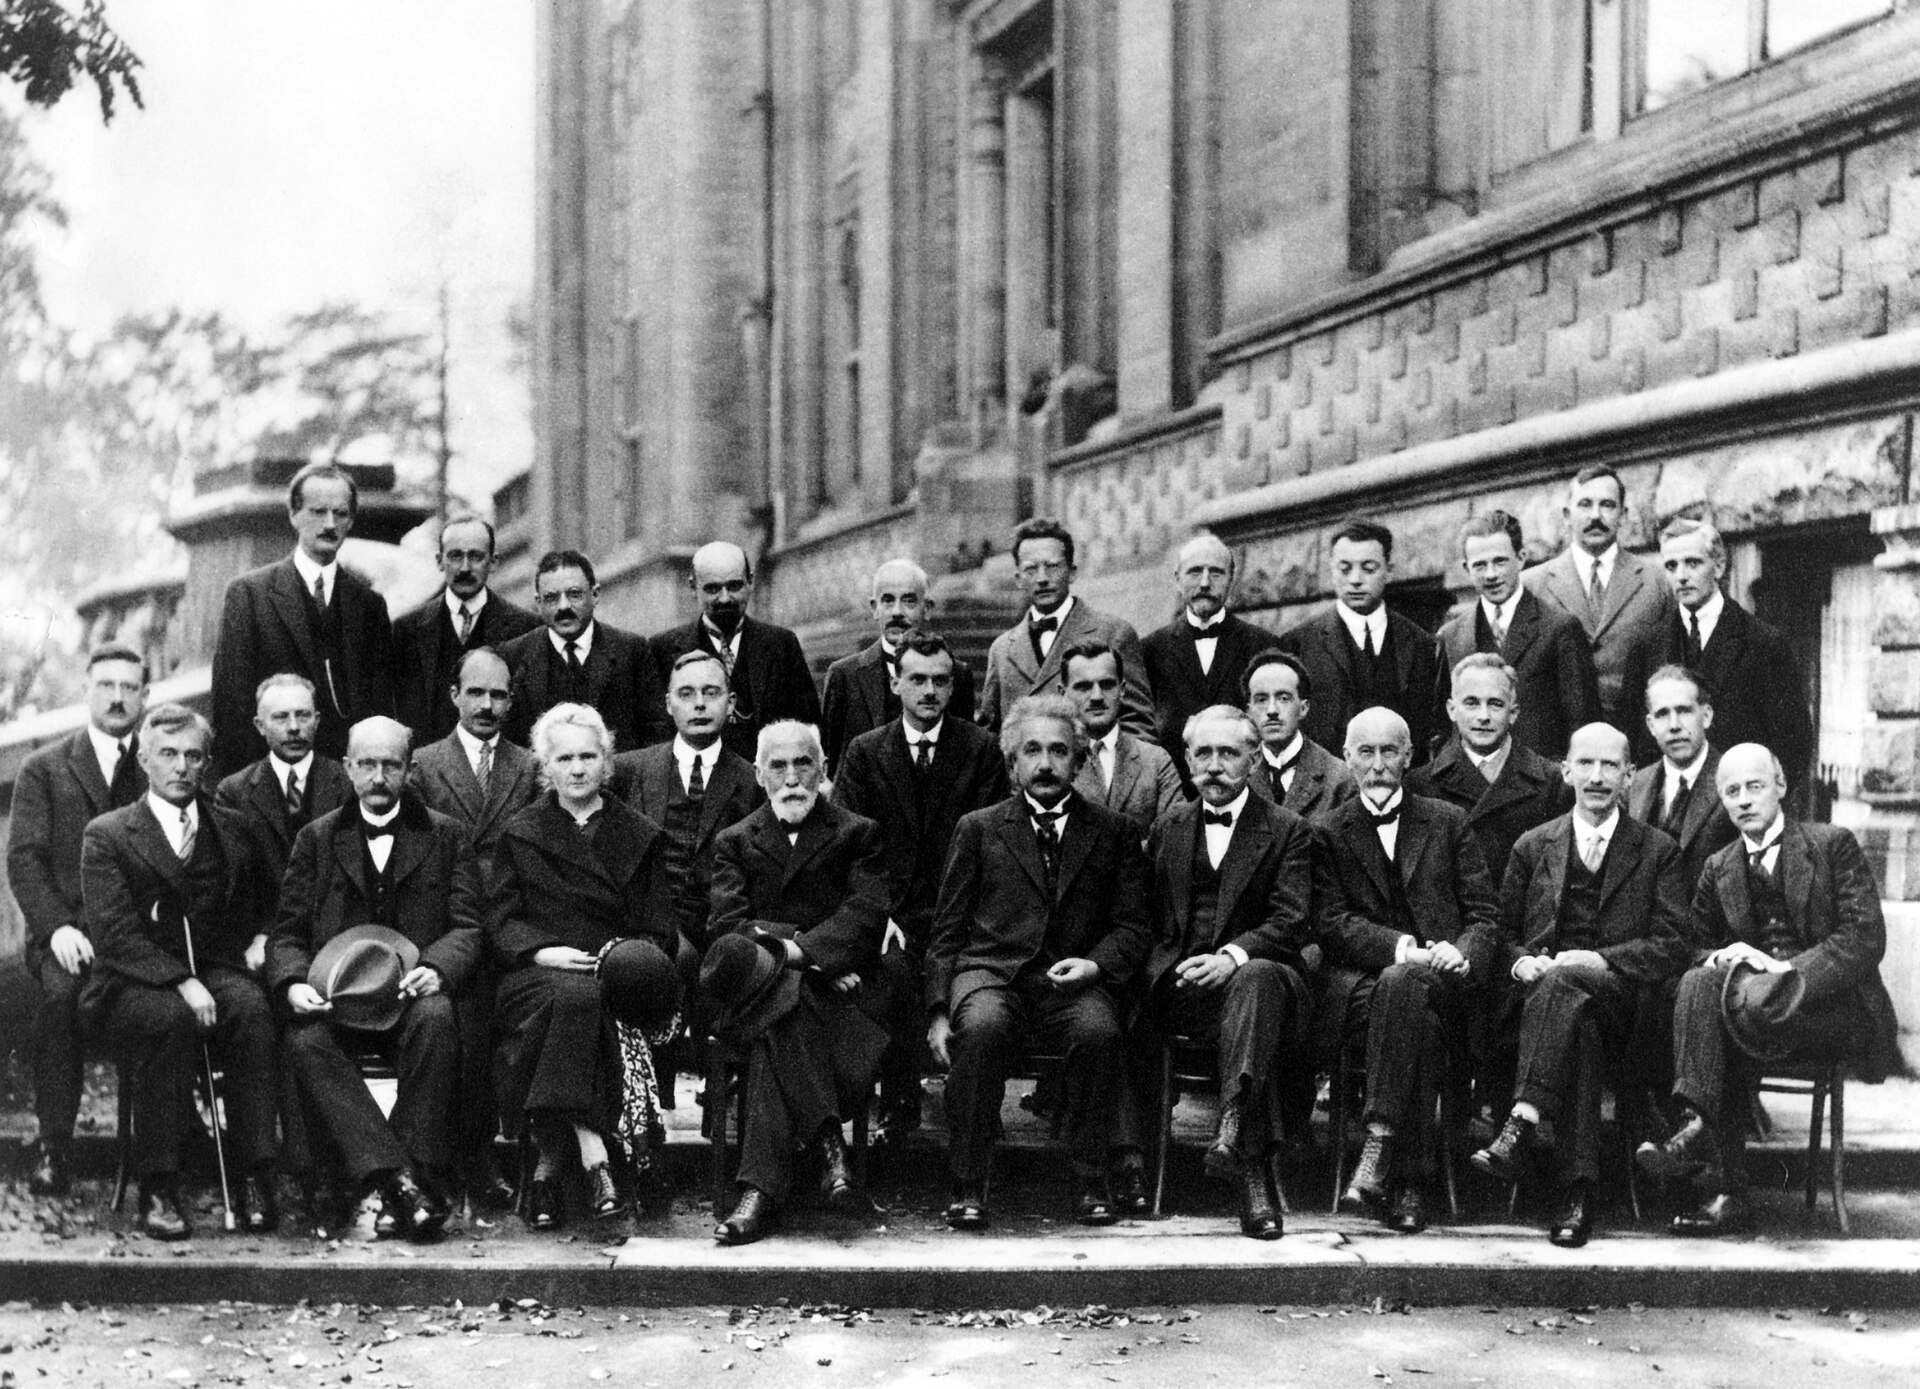
\includegraphics[width=\textwidth]{images/Solvay_conference_1927.jpg}
\end{figure}

\end{document}
